\chapter{Injection beam loss monitoring system}\label{sec:Injection bea loss monitoring system}

\section{Required performance}

At the SuperKEKB accelerator, the beam revolution period is approximately 10 us. Therefore, high time resolution is required to measure injection beam loss on a turn-by-turn basis. In addition, the sensors installed near the collimators are connected to readout boards via cables several hundreds meters long, resulting in signal attenuation. Thus, a sufficient high signal gain is required. Furthermore, the sensors have mo Sensor ust be radiation tolerant because the regions around the collimators are exposed to high radiation levels. 


\section{CLAWS sensor}
The CLAWS consists of plastic scintillator (3$\times$3 cm) and MPPC. 
The CLAWS sensor was originally developed to monitor radiation levels at the interaction region (IR) and for use in the beam-abort system. In recent years, the CLAWS sensors have been installed near the collimators, with their gain improved for use in the beam-abort system. The sensors have a time resolution of O(10 ns) and a gain of $10^5-10^6$, which are sufficient for measuring injection beam loss on a turn-by-turn basis. Since the radiation levels at the IR are significantly higher than those along the beam line, the sensor has demonstrated sufficient radiation tolerance for this application.
\begin{figure}
    \centering
    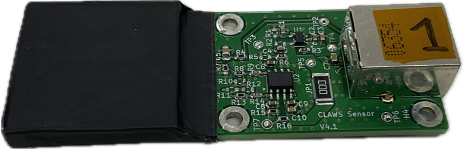
\includegraphics[width=0.6\columnwidth]{Figures/C04_Monitoring_system/CLAWS.png}
    \caption{CLAWS sensor}
    \label{fig:CLAWS}
\end{figure}

\section{Install position}


The CLAWS sensors are mounted on support structure approximately 1 m downstream of the collimators. Since radiation showers are expected to propagate parallel to the beam pipe, the sensors were installed so that the elevation was as small as possible. 
\begin{figure}
    \centering
    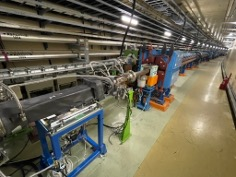
\includegraphics[width=0.6\columnwidth]{Figures/C04_Monitoring_system/install.png}
    \caption{CLAWS sensor install position}
    \label{fig:install_position}
\end{figure}


\section{Readout}

The CLAWS sigals are acquired synchronously with the 1 Hz prescaled injection kicker signal. The signals are transmitted through cables several hundreds meters long to the power supply buildings on the ground. Receiver boards installed in these buildings condition the signal before they are read by oscilloscopes. The oscilloscopes are controlled by PCs,  and waveform data covering 23 ms window after the trigger is acquired.

\section{Data correction, processing, recording}

The raw waveform data acquired oevr 23ms window consist of approximately 1 million samples, making it impractical to store all the raw data. Therefore, the following quantities are calculated from the raw waveforms and recorded instead: \\

1. Turn-by-turn beam loss : The raw waveform is integrated for each turn after applying a threshold to identify the beam loss signal.\\
2. Total beam loss per injection : The sum of the turn-by-turn beam loss values.\\
3. Beam loss accumulated before and after 1ms : The sum of the beam loss values from the injection trriger to 1ms and from 1ms to the end of the acquisition window, respectively.\\
4. Centroid of the beam loss duration : The time centroid of the beam loss signal for each injection.\\

These quantities are recorded as process valuables (PVs) in the Archiver, the data archiving system used at SuperKEKB. This allows the data to be accessed by users.